\begin{center}
  \textbf{Отчёт лабораторной работы №\envReportLabNumber}
\end{center}

\textbf{Тема}:
<<\envReportTitle>>

\textbf{Цель}:
изучить основы методов Machine Learning в контексте задачи
множественного регрессионного анализа,
приобрести навыки работы с методами Machine Learning в системе STATISTICA StatSoft,
осуществить обработку методами Machine Learning индивидуального набора данных и интерпретацию результатов.
% = = = = = = = = = = = = = = = =

\phantomsection
\addcontentsline{toc}{section}{Подготовка к лабораторной работе}

\begin{center}
  \textbf{Пробует пример по методичке}
\end{center}

Удаляю папку <<Statistica 10 RUS>>.

Запускаю Ststatistica\_10\_ru\_portable.exe.

\begin{center}
  \textbf{Файл данных}
\end{center}

Главная > Открыть $\bigtriangledown$ > Открыть папку примеров\\
> Z:$\backslash$MOD\_\_Examples$\backslash$Examples$\backslash$Datasets$\backslash$Poverty.sta
> Открыть. Результат на рисунке~\ref{fig:example_1}.

\begin{figure}[!h]
  \centering

  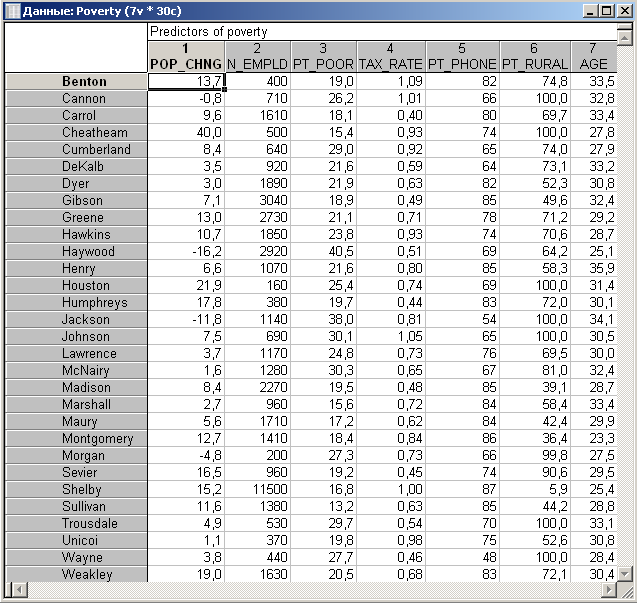
\includegraphics[height=15cm]
  {inc/example_1.PNG}

  \caption{q}

  \label{fig:example_1}
\end{figure}

\newpage

Данные > Спецификации > Все спецификации > OK 

Результаты на рисунках~\ref{fig:example_2}, \ref{fig:example_3}.

\begin{figure}[!h]
  \centering
  \begin{minipage}{0.49\textwidth}
    \centering

    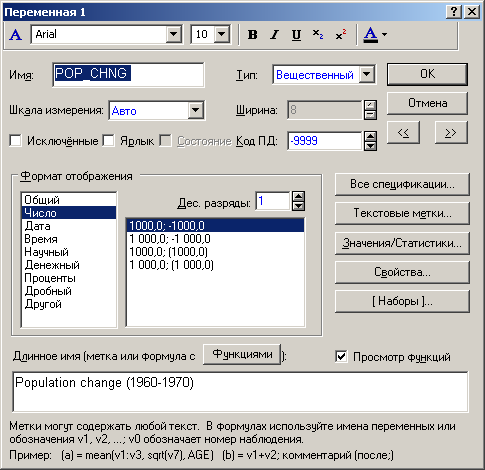
\includegraphics[height=6.5cm]
    {inc/example_2.PNG}

    \caption{q}
    \label{fig:example_2}
  \end{minipage}
  \begin{minipage}{0.49\textwidth}
    \centering

    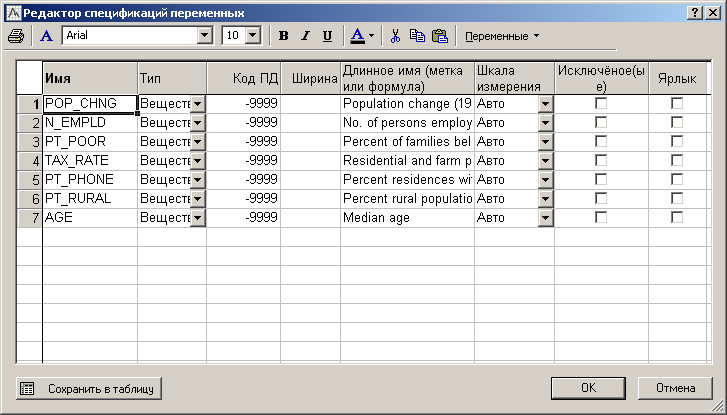
\includegraphics[width=0.99\textwidth]
    {inc/example_3.PNG}

    \caption{q}
    \label{fig:example_3}
  \end{minipage}
\end{figure}

\begin{center}
  \textbf{Начало анализа}
\end{center}

Анализ > Множественная регрессия > Быстрый > Переменные\\
> Зависимые переменные > 3-PT\_POOR\\
> Независимые переменные > Ctrl 1-POP\_CHNG, Ctrl 2-N\_EMPLD,
Ctrl 4-TAX\_RATE, Ctrl 5-PT\_PHONE, Ctrl 6-PT\_RURAL, Ctrl 7-AGE\\
> Переменные > OK > Дополнительно > Показывать опис. мтатист., корр. матрицы. > OK\\
> Быстрый > Средние и ст. отклонения

Результаты на рисунках~\ref{fig:example_4}, \ref{fig:example_5}, \ref{fig:example_6}.

\begin{figure}[!h]
  \centering
  \begin{minipage}{0.36\textwidth}
    \centering

    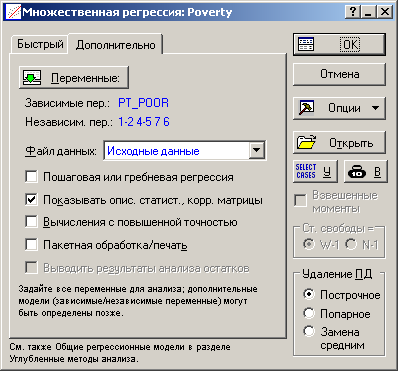
\includegraphics[width=0.99\textwidth]
    {inc/example_4.PNG}

    \caption{q}
    \label{fig:example_4}
  \end{minipage}
  \begin{minipage}{0.36\textwidth}
    \centering

    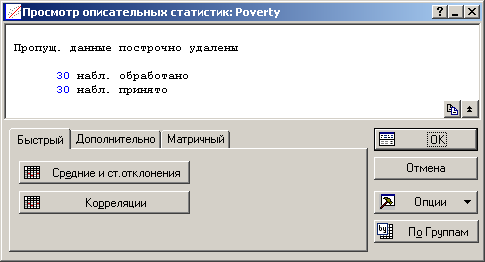
\includegraphics[width=0.99\textwidth]
    {inc/example_5.PNG}

    \caption{q}
    \label{fig:example_5}
  \end{minipage}
  \begin{minipage}{0.24\textwidth}
    \centering

    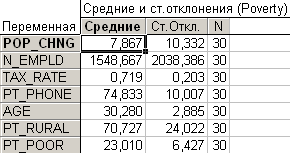
\includegraphics[width=0.99\textwidth]
    {inc/example_6.PNG}

    \caption{q}
    \label{fig:example_6}
  \end{minipage}
\end{figure}

\newpage

\begin{center}
  \textbf{Распределение переменных}
\end{center}

Графики > 2М Гистограмма > Дополнительно > Интервалы > Категории > 16 > OK
> 3-PT\_POOR > OK > OK. Результаты на рисунках~\ref{fig:example_7}, \ref{fig:example_8}, \ref{fig:example_9}.

\begin{figure}[!h]
  \centering
  \begin{minipage}{0.49\textwidth}
    \centering

    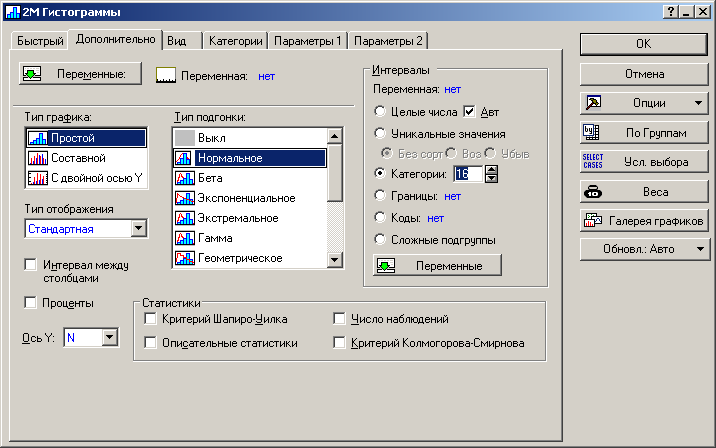
\includegraphics[height=5cm]
    {inc/example_7.PNG}

    \caption{q}
    \label{fig:example_7}
  \end{minipage}
  \begin{minipage}{0.49\textwidth}
    \centering

    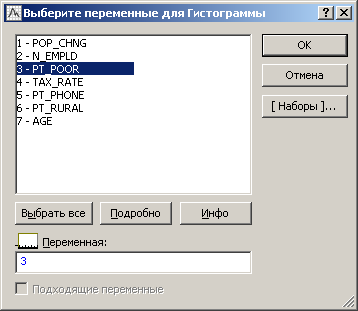
\includegraphics[height=5cm]
    {inc/example_8.PNG}

    \caption{q}
    \label{fig:example_8}
  \end{minipage}
\end{figure}

\begin{figure}[!h]
  \centering

  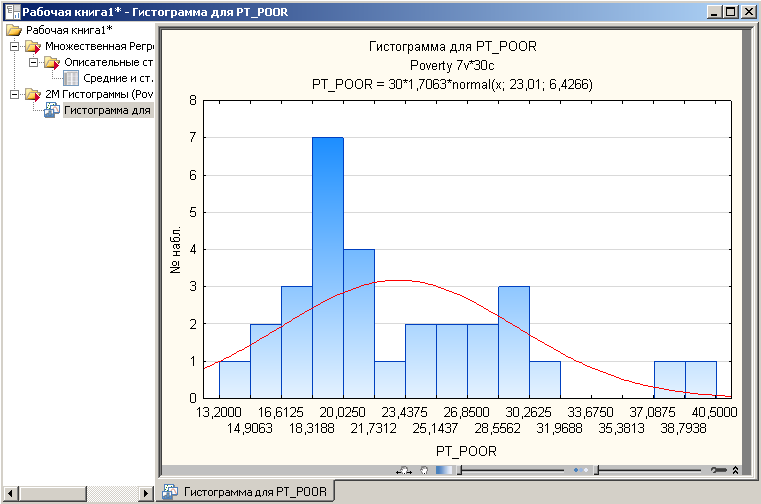
\includegraphics[width=11cm]
  {inc/example_9.PNG}

  \caption{q}

  \label{fig:example_9}
\end{figure}

Просмотр описательной статистик: Proverty
> Дополнительно > Диаграмма размаха > 3 — PT\_POOR > OK > Медиана/Квартиль/Размах > OK

Результаты на рисунках~\ref{fig:example_10}, \ref{fig:example_11}, \ref{fig:example_12}, \ref{fig:example_13}.

\begin{figure}[!h]
  \centering
  \begin{minipage}{0.32\textwidth}
    \centering

    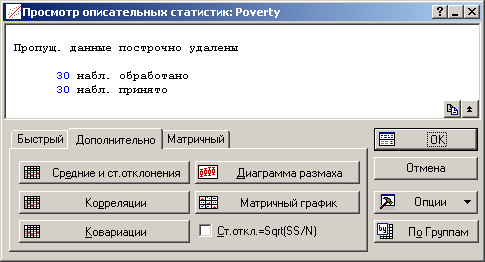
\includegraphics[width=0.99\textwidth]
    {inc/example_10.PNG}

    \caption{q}
    \label{fig:example_10}
  \end{minipage}
  \begin{minipage}{0.32\textwidth}
    \centering

    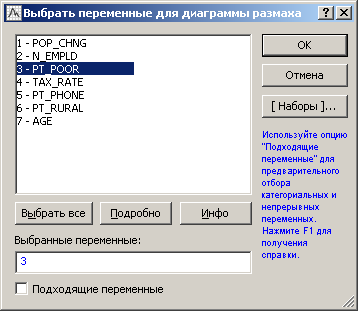
\includegraphics[width=0.99\textwidth]
    {inc/example_11.PNG}

    \caption{q}
    \label{fig:example_11}
  \end{minipage}
  \begin{minipage}{0.32\textwidth}
    \centering

    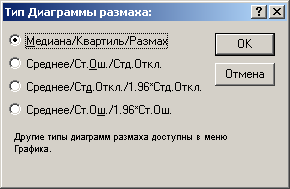
\includegraphics[width=0.99\textwidth]
    {inc/example_12.PNG}

    \caption{q}
    \label{fig:example_12}
  \end{minipage}
\end{figure}

\begin{figure}[!h]
  \centering

  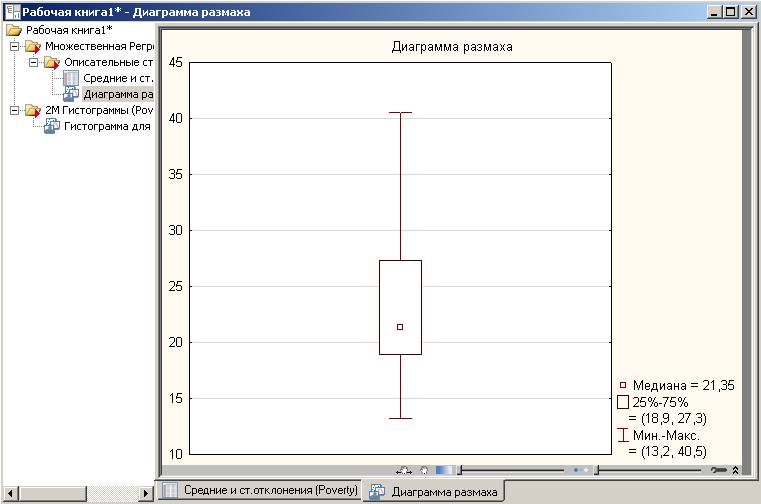
\includegraphics[width=11cm]
  {inc/example_13.PNG}

  \caption{q}

  \label{fig:example_13}
\end{figure}

\newpage

\begin{center}
  \textbf{Диаграммы рассеяния}
\end{center}

Просмотр описательной статистик: Proverty > Быстрый > Корреляции

Результаты на рисунках~\ref{fig:example_14}, \ref{fig:example_15}.

\begin{figure}[!h]
  \centering
  \begin{minipage}{0.29\textwidth}
    \centering

    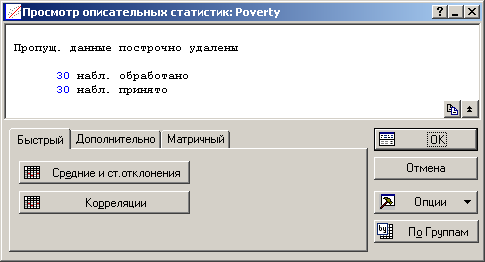
\includegraphics[width=0.99\textwidth]
    {inc/example_14.PNG}

    \caption{q}
    \label{fig:example_14}
  \end{minipage}
  \begin{minipage}{0.69\textwidth}
    \centering

    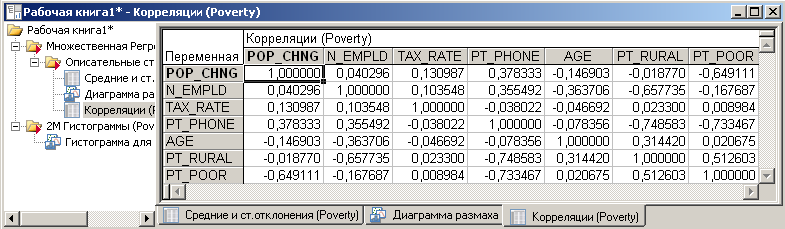
\includegraphics[width=0.99\textwidth]
    {inc/example_15.PNG}

    \caption{q}
    \label{fig:example_15}
  \end{minipage}
\end{figure}

Просмотр описательной статистик: Proverty > Дополнительно > Матричный график > 1-2 4-7 3 > OK

Результаты на рисунках~\ref{fig:example_16}, \ref{fig:example_17}, \ref{fig:example_18}.

\begin{figure}[!h]
  \centering
  \begin{minipage}{0.49\textwidth}
    \centering

    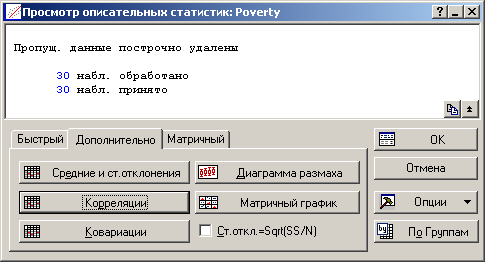
\includegraphics[height=5cm]
    {inc/example_16.PNG}

    \caption{q}
    \label{fig:example_16}
  \end{minipage}
  \begin{minipage}{0.49\textwidth}
    \centering

    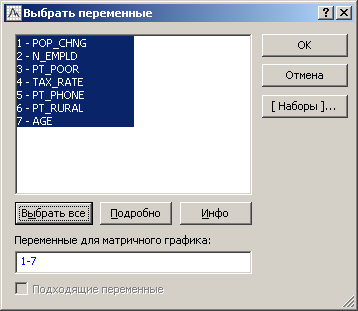
\includegraphics[height=5cm]
    {inc/example_17.PNG}

    \caption{q}
    \label{fig:example_17}
  \end{minipage}
\end{figure}

\begin{figure}[!h]
  \centering

  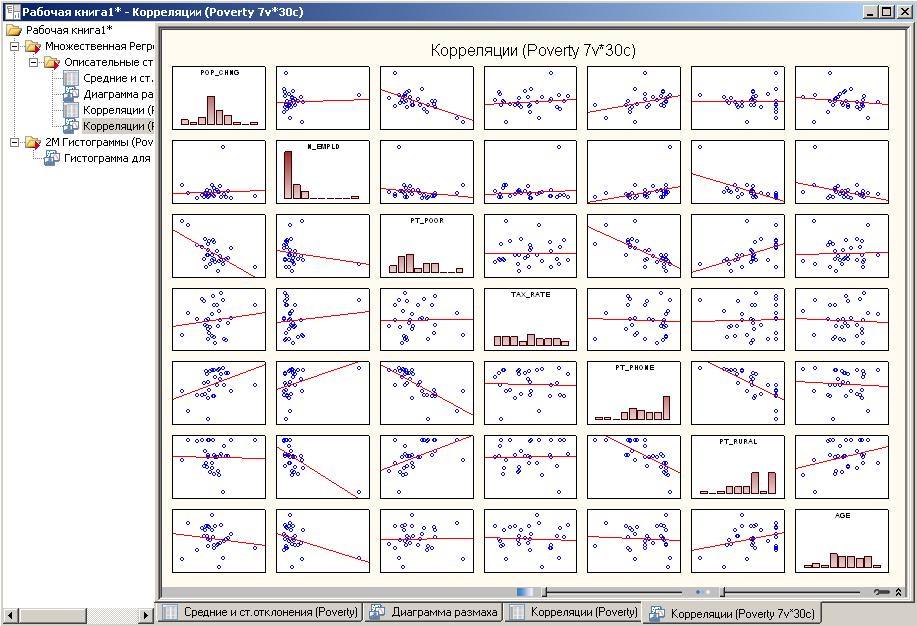
\includegraphics[height=9.6cm]
  {inc/example_18.PNG}

  \caption{q}

  \label{fig:example_18}
\end{figure}

\newpage

\begin{center}
  \textbf{Определение множественной регрессии. Просмотр результатов}
\end{center}

Просмотр описательной статистик: Proverty > OK

Результат на рисунке~\ref{fig:example_19}.

\begin{figure}[!h]
  \centering

  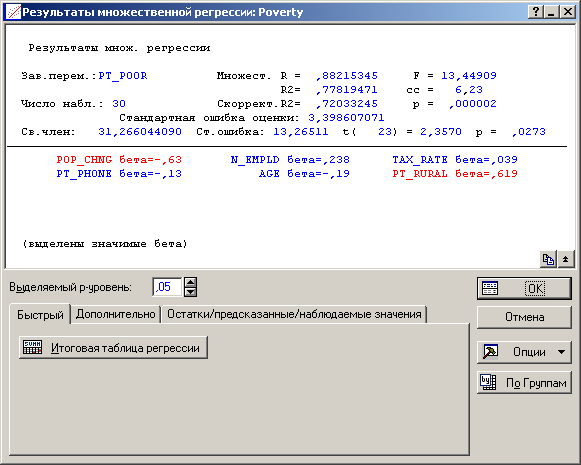
\includegraphics[height=8cm]
  {inc/example_19.PNG}

  \caption{q}

  \label{fig:example_19}
\end{figure}

\newpage

\begin{center}
  \textbf{Коэффициенты регрессии}
\end{center}

Результаты множественной регрессии: Proverty > Быстрый > Итоговая таблица регрессии.

Результат на рисунке~\ref{fig:example_20}.

\begin{figure}[!h]
  \centering

  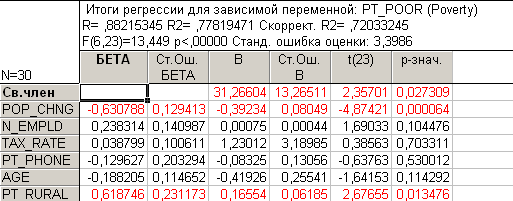
\includegraphics[width=12cm]
  {inc/example_20.PNG}

  \caption{q}

  \label{fig:example_20}
\end{figure}

\begin{center}
  \textbf{Частичные корреляции}
\end{center}

Результаты множественной регрессии: Provety > Дополнительно > Частные корреляции

Результаты на рисунках~\ref{fig:example_21}, \ref{fig:example_22}.

\begin{figure}[!h]
  \centering
  \begin{minipage}{0.49\textwidth}
    \centering

    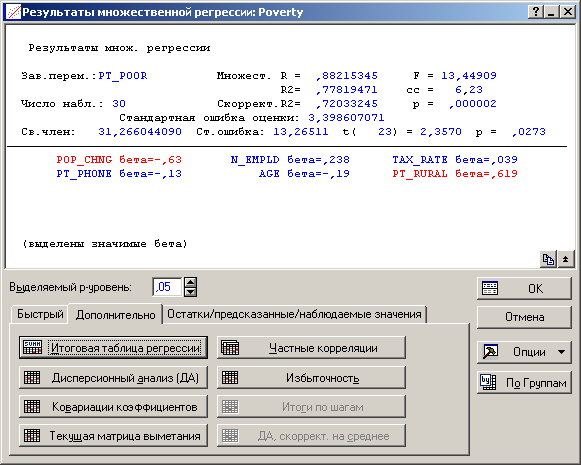
\includegraphics[height=5cm]
    {inc/example_21.PNG}

    \caption{q}
    \label{fig:example_21}
  \end{minipage}
  \begin{minipage}{0.49\textwidth}
    \centering

    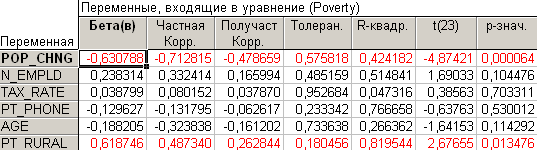
\includegraphics[width=0.99\textwidth]
    {inc/example_22.PNG}

    \caption{q}
    \label{fig:example_22}
  \end{minipage}
\end{figure}

\newpage

\begin{center}
  \textbf{Анализ остатков}
\end{center}

Результаты множественной регрессии: Provety > Остатки/предсказанные/наблюдаемые значения > Анализ остатков > Быстрый > Остатки и предсказанные

Результаты на рисунках~\ref{fig:example_23}, \ref{fig:example_24}, \ref{fig:example_25}.

\begin{figure}[!h]
  \centering
  \begin{minipage}{0.29\textwidth}
    \centering

    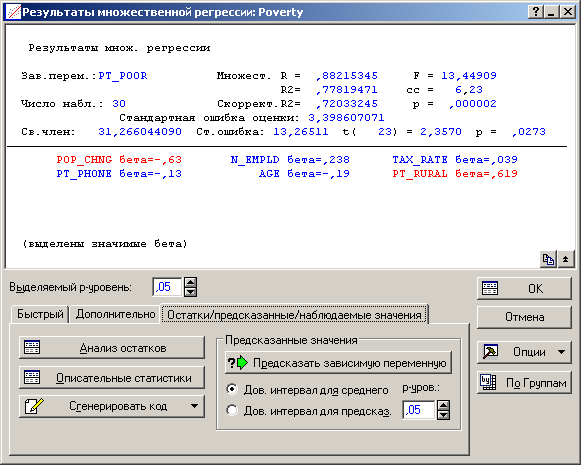
\includegraphics[height=5.3cm]
    {inc/example_23.PNG}

    \caption{q}
    \label{fig:example_23}
  \end{minipage}
  \begin{minipage}{0.69\textwidth}
    \centering

    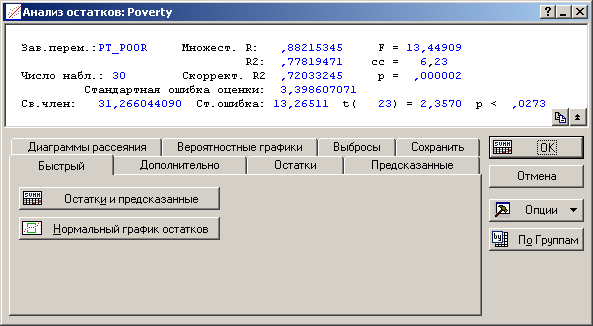
\includegraphics[height=5.3cm]
    {inc/example_24.PNG}

    \caption{q}
    \label{fig:example_24}
  \end{minipage}
\end{figure}

\begin{figure}[!h]
  \centering

  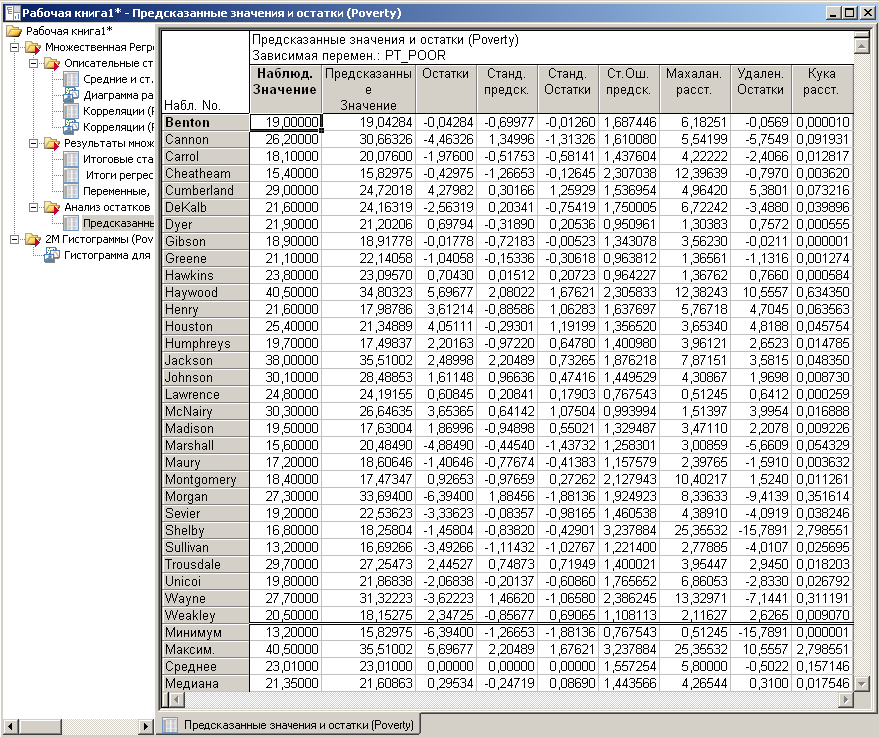
\includegraphics[width=14cm]
  {inc/example_25.PNG}

  \caption{q}

  \label{fig:example_25}
\end{figure}

\newpage

\begin{center}
  \textbf{График случайных остатков}
\end{center}

Анализ остатков: Poverty > Остатки > Построчн. графики остатков

Результаты на рисунках~\ref{fig:example_27}, \ref{fig:example_28}.

\begin{figure}[!h]
  \centering

  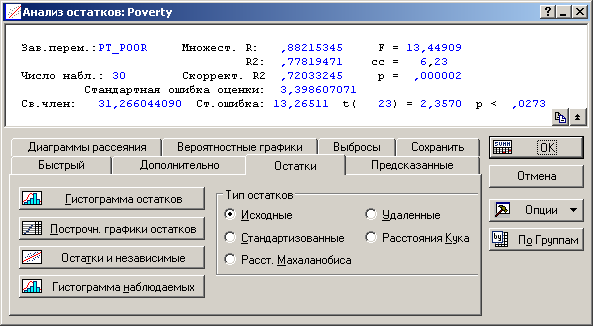
\includegraphics[height=8cm]
  {inc/example_27.PNG}

  \caption{q}

  \label{fig:example_27}
\end{figure}

\begin{figure}[!h]
  \centering

  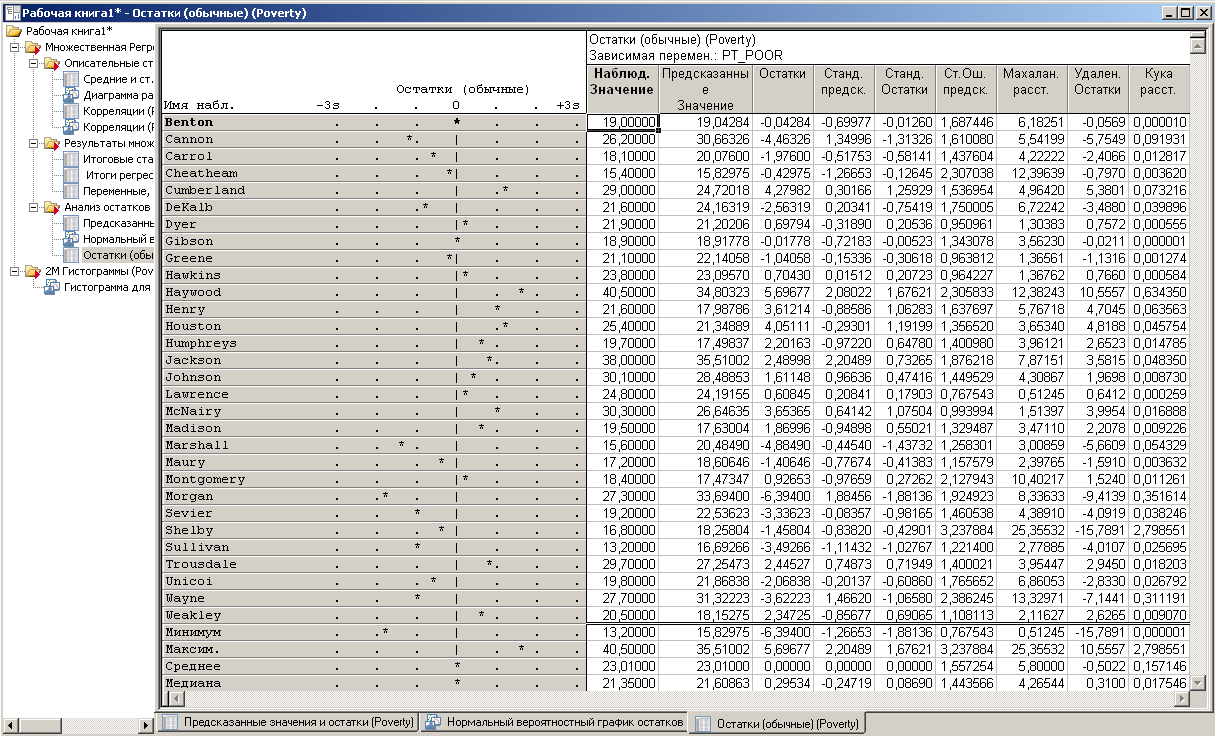
\includegraphics[width=17cm]
  {inc/example_28.PNG}

  \caption{q}

  \label{fig:example_28}
\end{figure}

\newpage

\textbf{График случайных выбросов}

Анализ остатков: Poverty > Выбросы > Построчн. график выбросов

Результаты на рисунках~\ref{fig:example_29}, \ref{fig:example_30}.

\begin{figure}[!h]
  \centering
  \begin{minipage}{0.49\textwidth}
    \centering

    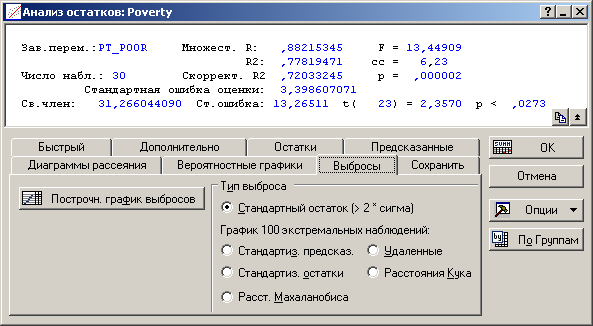
\includegraphics[height=4.5cm]
    {inc/example_29.PNG}

    \caption{q}
    \label{fig:example_29}
  \end{minipage}
  \begin{minipage}{0.49\textwidth}
    \centering

    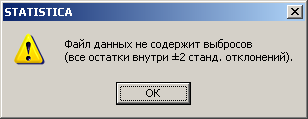
\includegraphics[width=0.99\textwidth]
    {inc/example_30.PNG}

    \caption{q}
    \label{fig:example_30}
  \end{minipage}
\end{figure}

\textbf{Расстояние Махаланобиса (Mahalanobis distances)}

Анализ остатков: Poverty > Выбросы\\
> График 100 экстремальных наблюдений > Расст. Махаланобиса\\
> Построчн. график выбросов

Результаты на рисунках~\ref{fig:example_31}, \ref{fig:example_32}.

\begin{figure}[!h]
  \centering

  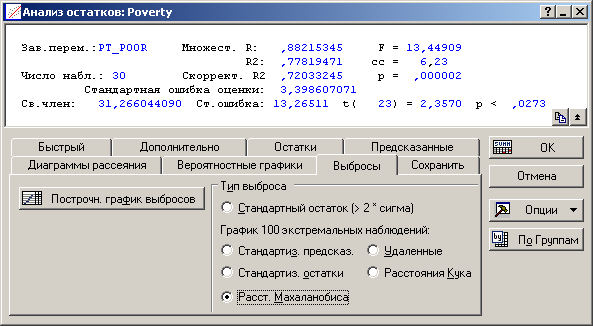
\includegraphics[height=4cm]
  {inc/example_31.PNG}

  \caption{q}

  \label{fig:example_31}
\end{figure}

\begin{figure}[!h]
  \centering

  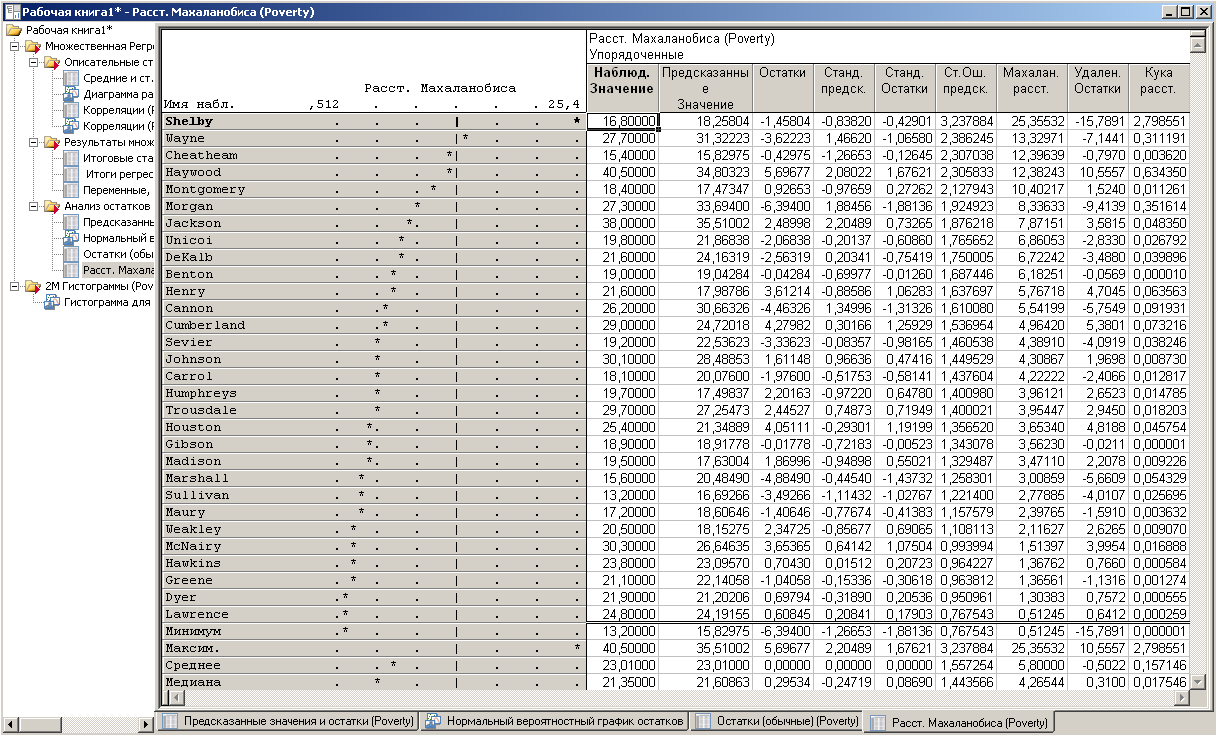
\includegraphics[width=13cm]
  {inc/example_32.PNG}

  \caption{q}

  \label{fig:example_32}
\end{figure}

\newpage

\textbf{Удаленные остатки}

Анализ остатков: Poverty > Диаграммы рассеяния >  Предсказание и остатки

Результаты на рисунках~\ref{fig:example_33}, \ref{fig:example_34}.

\begin{figure}[!h]
  \centering

  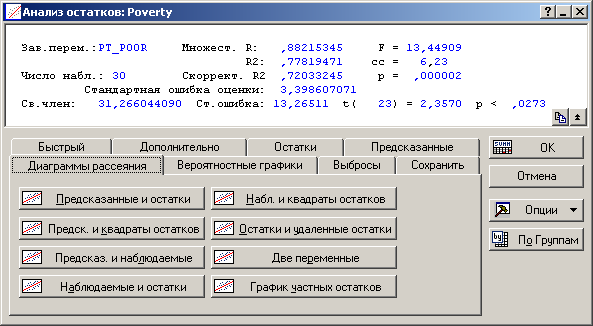
\includegraphics[height=8cm]
  {inc/example_33.PNG}

  \caption{q}

  \label{fig:example_33}
\end{figure}

\begin{figure}[!h]
  \centering

  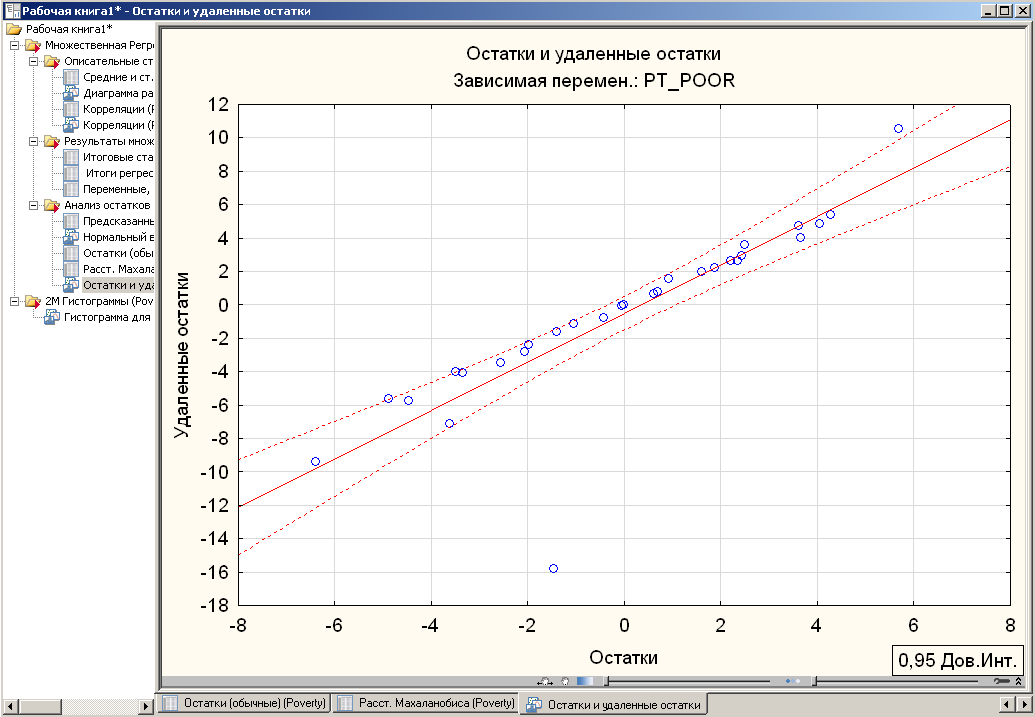
\includegraphics[width=16cm]
  {inc/example_34.PNG}

  \caption{q}

  \label{fig:example_34}
\end{figure}

\newpage

\textbf{Графики нормальной вероятности}

Анализ остатков: Poverty > Вероятностные графики > Нормальный график остатков

Результаты на рисунках~\ref{fig:example_35}, \ref{fig:example_36}.

\begin{figure}[!h]
  \centering

  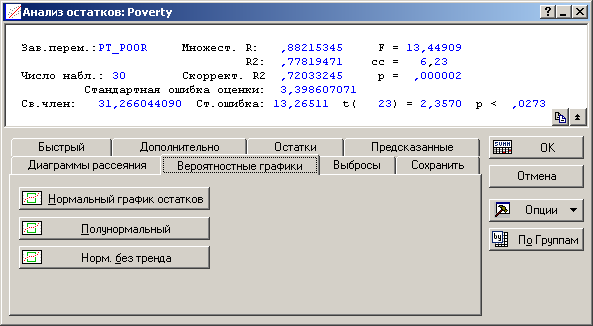
\includegraphics[height=8cm]
  {inc/example_35.PNG}

  \caption{q}

  \label{fig:example_35}
\end{figure}

\begin{figure}[!h]
  \centering

  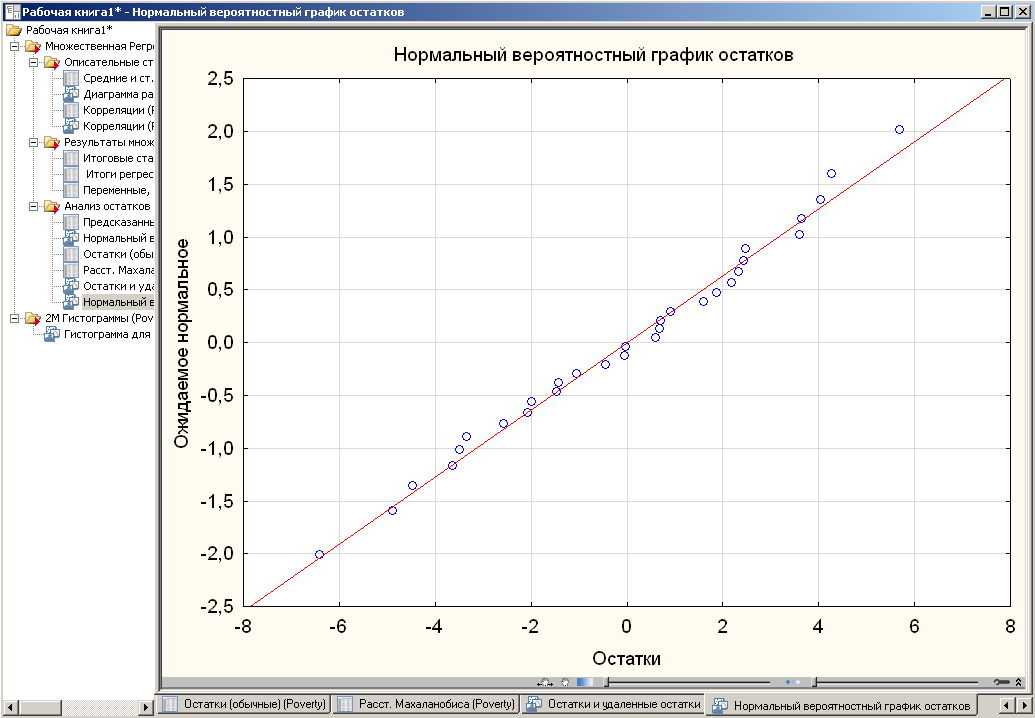
\includegraphics[width=16cm]
  {inc/example_36.PNG}

  \caption{q}

  \label{fig:example_36}
\end{figure}

\newpage

\begin{center}
  \textbf{Вариант 5}
\end{center}

Удаляю папку <<Statistica 10 RUS>>.

Запускаю Ststatistica\_10\_ru\_portable.exe.

\begin{center}
  \textbf{Файл данных}
\end{center}

Главная > Открыть > <<Fish for vars 1-5.xls>> > Открыть \\
> Импортировать выбранный лист в Таблицу данных > Var5 > OK \\
> Имена переменных из первой строки\\
> Имена наблюдений из первого столбца > OK

Результат на рисунке~\ref{fig:var5__1}.

\begin{figure}[!h]
  \centering

  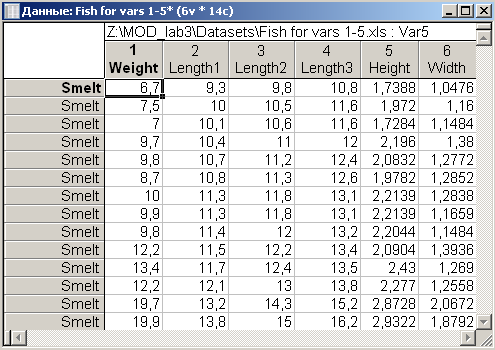
\includegraphics[height=7cm]
  {inc/var5__1.PNG}

  \caption{q}

  \label{fig:var5__1}
\end{figure}

Данные > Спецификации > Все спецификации > OK 

Результаты на рисунках~\ref{fig:var5__2}, \ref{fig:var5__3}.

\begin{figure}[!h]
  \centering
  \begin{minipage}{0.49\textwidth}
    \centering

    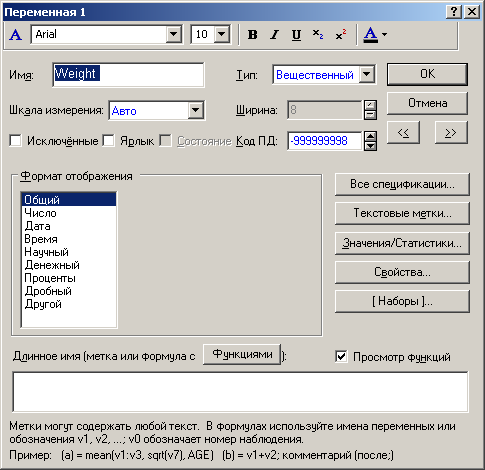
\includegraphics[height=6.5cm]
    {inc/var5__2.PNG}

    \caption{q}
    \label{fig:var5__2}
  \end{minipage}
  \begin{minipage}{0.49\textwidth}
    \centering

    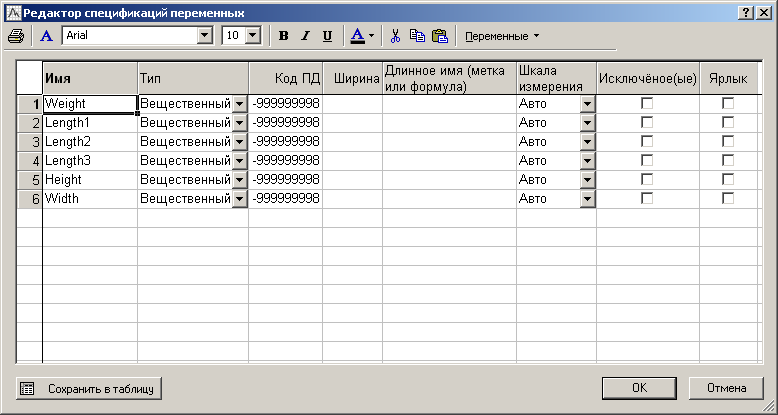
\includegraphics[width=0.99\textwidth]
    {inc/var5__3.PNG}

    \caption{q}
    \label{fig:var5__3}
  \end{minipage}
\end{figure}

\newpage

\begin{center}
  \textbf{Начало анализа}
\end{center}

Анализ > Множественная регрессия > Быстрый > Переменные\\
> Зависимые переменные > 1 > Независимые переменные > 2-6 > OK\\
> Дополнительно > Показывать опис. мтатист., корр. матрицы. > OK\\
> Быстрый > Средние и ст. отклонения

Результаты на рисунках~\ref{fig:var5__4}, \ref{fig:var5__5}, \ref{fig:var5__6}, \ref{fig:var5__7}.

\begin{figure}[!h]
  \centering
  \begin{minipage}{0.49\textwidth}
    \centering

    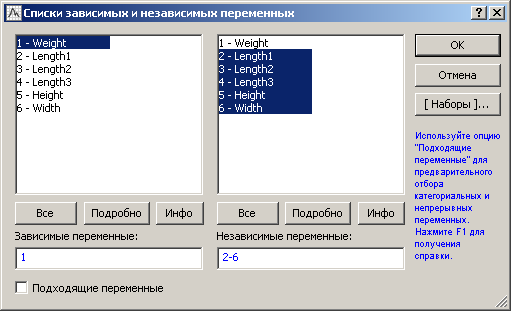
\includegraphics[width=0.99\textwidth]
    {inc/var5__4.PNG}

    \caption{q}
    \label{fig:var5__4}
  \end{minipage}
  \begin{minipage}{0.49\textwidth}
    \centering

    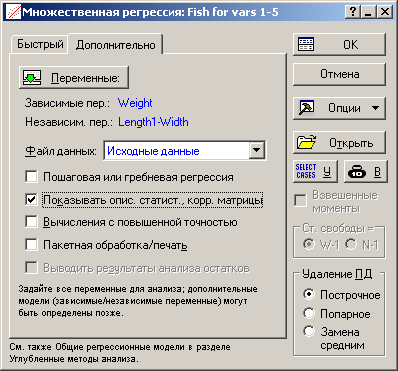
\includegraphics[width=0.99\textwidth]
    {inc/var5__5.PNG}

    \caption{q}
    \label{fig:var5__5}
  \end{minipage}
\end{figure}

\begin{figure}[!h]
  \centering
  \begin{minipage}{0.49\textwidth}
    \centering

    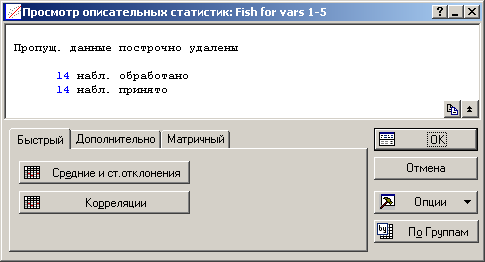
\includegraphics[width=0.99\textwidth]
    {inc/var5__6.PNG}

    \caption{q}
    \label{fig:var5__6}
  \end{minipage}
  \begin{minipage}{0.49\textwidth}
    \centering

    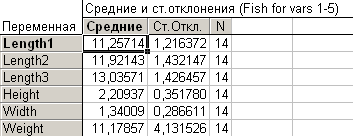
\includegraphics[width=0.99\textwidth]
    {inc/var5__7.PNG}

    \caption{q}
    \label{fig:var5__7}
  \end{minipage}
\end{figure}

\newpage

\begin{center}
  \textbf{Распределение переменных}
\end{center}

Графики > 2М Гистограмма > Дополнительно > Интервалы > Категории > 16 > OK
> Переменные > 1 > OK > OK. Результаты на рисунках~\ref{fig:var5__8}, \ref{fig:var5__9}, \ref{fig:var5__10}.

\begin{figure}[!h]
  \centering
  \begin{minipage}{0.49\textwidth}
    \centering

    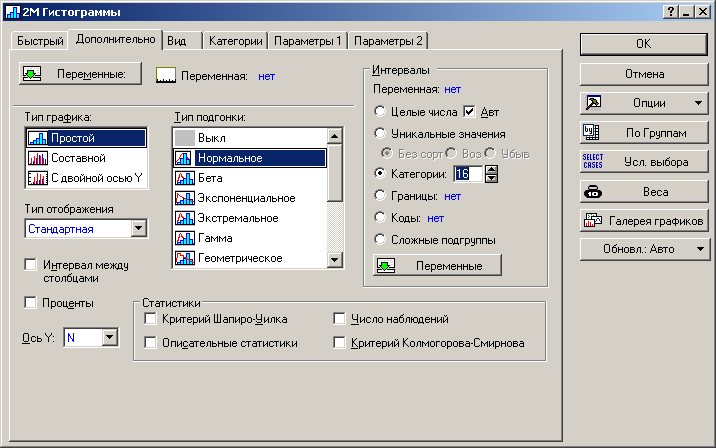
\includegraphics[height=5cm]
    {inc/var5__8.PNG}

    \caption{q}
    \label{fig:var5__8}
  \end{minipage}
  \begin{minipage}{0.49\textwidth}
    \centering

    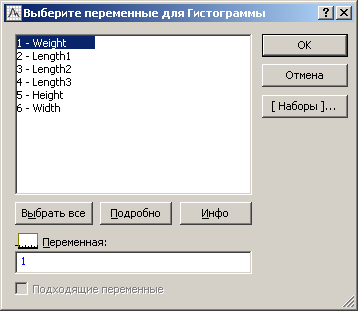
\includegraphics[height=5cm]
    {inc/var5__9.PNG}

    \caption{q}
    \label{fig:var5__9}
  \end{minipage}
\end{figure}

\begin{figure}[!h]
  \centering

  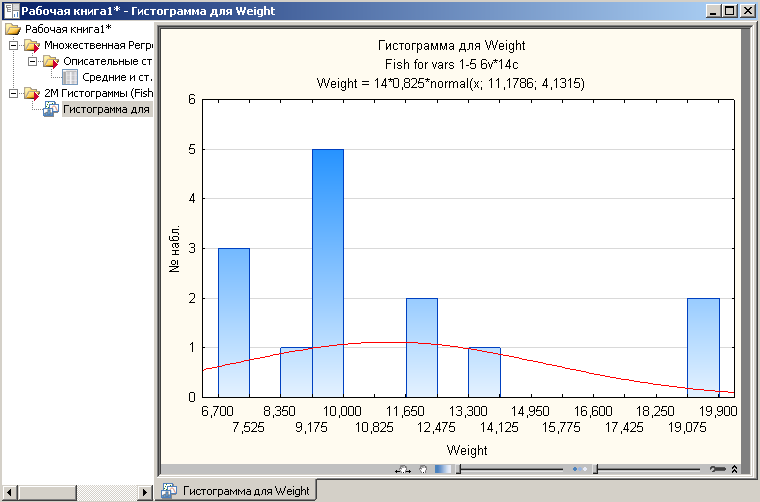
\includegraphics[width=11cm]
  {inc/var5__10.PNG}

  \caption{q}

  \label{fig:var5__10}
\end{figure}

Просмотр описательной статистик: Fish for var 1-5
> Дополнительно > Диаграмма размаха > 1 > OK > Медиана/Квартиль/Размах > OK

Результаты на рисунках~\ref{fig:var5__11}, \ref{fig:var5__12}, \ref{fig:var5__13}, \ref{fig:var5__14}.

\begin{figure}[!h]
  \centering
  \begin{minipage}{0.32\textwidth}
    \centering

    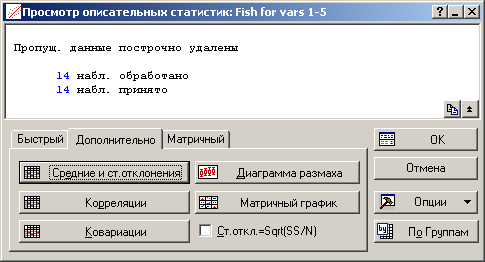
\includegraphics[width=0.99\textwidth]
    {inc/var5__11.PNG}

    \caption{q}
    \label{fig:var5__11}
  \end{minipage}
  \begin{minipage}{0.32\textwidth}
    \centering

    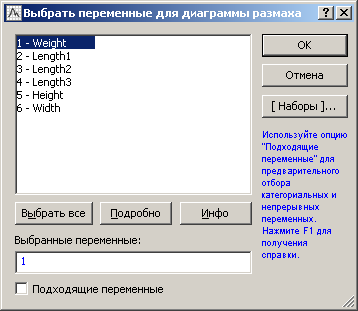
\includegraphics[width=0.99\textwidth]
    {inc/var5__12.PNG}

    \caption{q}
    \label{fig:var5__12}
  \end{minipage}
  \begin{minipage}{0.32\textwidth}
    \centering

    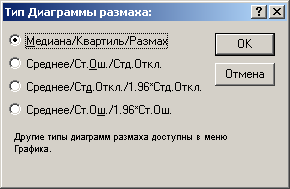
\includegraphics[width=0.99\textwidth]
    {inc/var5__13.PNG}

    \caption{q}
    \label{fig:var5__13}
  \end{minipage}
\end{figure}

\begin{figure}[!h]
  \centering

  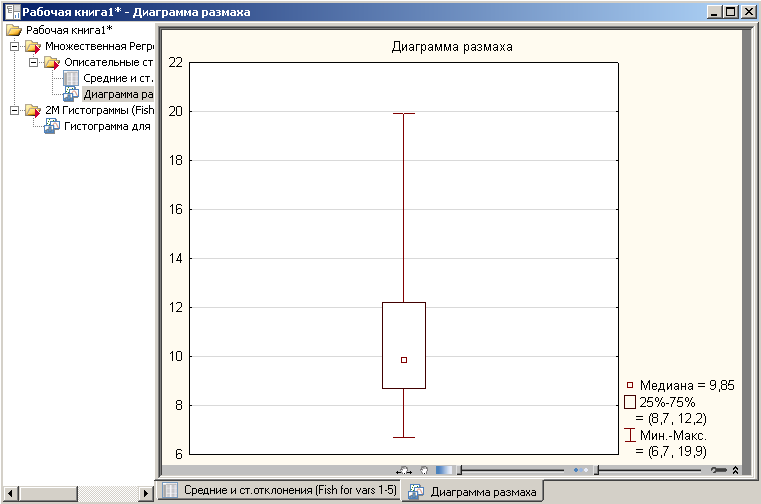
\includegraphics[width=11cm]
  {inc/var5__14.PNG}

  \caption{q}

  \label{fig:var5__14}
\end{figure}

\newpage

\begin{center}
  \textbf{Диаграммы рассеяния}
\end{center}

Просмотр описательной статистик: Fish for var 1-5 > Быстрый > Корреляции

Результаты на рисунках~\ref{fig:var5__15}, \ref{fig:var5__16}.

\begin{figure}[!h]
  \centering
  \begin{minipage}{0.29\textwidth}
    \centering

    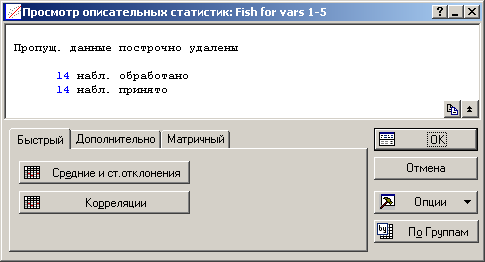
\includegraphics[width=0.99\textwidth]
    {inc/var5__15.PNG}

    \caption{q}
    \label{fig:var5__15}
  \end{minipage}
  \begin{minipage}{0.69\textwidth}
    \centering

    \includegraphics[width=0.99\textwidth]
    {inc/var5__16.PNG}

    \caption{q}
    \label{fig:var5__16}
  \end{minipage}
\end{figure}

Просмотр описательной статистик: Fish for var 1-5 > Дополнительно > Матричный график > 2-6 1 > OK

Результаты на рисунках~\ref{fig:var5__17}, \ref{fig:var5__18}, \ref{fig:var5__19}.

\begin{figure}[!h]
  \centering
  \begin{minipage}{0.49\textwidth}
    \centering

    \includegraphics[height=5cm]
    {inc/var5__17.PNG}

    \caption{q}
    \label{fig:var5__17}
  \end{minipage}
  \begin{minipage}{0.49\textwidth}
    \centering

    \includegraphics[height=5cm]
    {inc/var5__18.PNG}

    \caption{q}
    \label{fig:var5__18}
  \end{minipage}
\end{figure}

\begin{figure}[!h]
  \centering

  \includegraphics[height=9.6cm]
  {inc/var5__19.PNG}

  \caption{q}

  \label{fig:var5__19}
\end{figure}

\newpage

\begin{center}
  \textbf{Определение множественной регрессии. Просмотр результатов}
\end{center}

Просмотр описательной статистик: Fish for var 1-5 > OK

Результат на рисунке~\ref{fig:var5__20}.

\begin{figure}[!h]
  \centering

  \includegraphics[height=8cm]
  {inc/var5__20.PNG}

  \caption{q}

  \label{fig:var5__20}
\end{figure}

\newpage

\begin{center}
  \textbf{Коэффициенты регрессии}
\end{center}

Результаты множественной регрессии: Fish for var 1-5 > Быстрый > Итоговая таблица регрессии.

Результат на рисунке~\ref{fig:var5__21}.

\begin{figure}[!h]
  \centering

  \includegraphics[width=12cm]
  {inc/var5__21.PNG}

  \caption{q}

  \label{fig:var5__21}
\end{figure}

\begin{center}
  \textbf{Частичные корреляции}
\end{center}

Результаты множественной регрессии: Fish for var 1-5 > Дополнительно > Частные корреляции

Результаты на рисунках~\ref{fig:var5__22}, \ref{fig:var5__23}.

\begin{figure}[!h]
  \centering
  \begin{minipage}{0.49\textwidth}
    \centering

    \includegraphics[height=5cm]
    {inc/var5__22.PNG}

    \caption{Результаты множественной регрессии}
    \label{fig:var5__22}
  \end{minipage}
  \begin{minipage}{0.49\textwidth}
    \centering

    \includegraphics[width=0.99\textwidth]
    {inc/var5__23.PNG}

    \caption{Таблица}
    \label{fig:var5__23}
  \end{minipage}
\end{figure}

\newpage

\begin{center}
  \textbf{Анализ остатков}
\end{center}

Результаты множественной регрессии: Fish for var 1-5 > Остатки/предсказанные/наблюдаемые значения > Анализ остатков > Быстрый > Остатки и предсказанные

Результаты на рисунках~\ref{fig:var5__24}, \ref{fig:var5__25}, \ref{fig:var5__26}.

\begin{figure}[!h]
  \centering
  \begin{minipage}{0.29\textwidth}
    \centering

    \includegraphics[height=5.3cm]
    {inc/var5__24.PNG}

    \caption{Результаты множественной регрессии}
    \label{fig:var5__24}
  \end{minipage}
  \begin{minipage}{0.69\textwidth}
    \centering

    \includegraphics[height=5.3cm]
    {inc/var5__25.PNG}

    \caption{Анализ остатков}
    \label{fig:var5__25}
  \end{minipage}
\end{figure}

\begin{figure}[!h]
  \centering

  \includegraphics[width=14cm]
  {inc/var5__26.PNG}

  \caption{Предсказанные значения и остатки}

  \label{fig:var5__26}
\end{figure}

\newpage

\begin{center}
  \textbf{График случайных остатков}
\end{center}

Анализ остатков: Fish for var 1-5 > Остатки > Построчн. графики остатков

Результаты на рисунках~\ref{fig:var5__27}, \ref{fig:var5__28}.

\begin{figure}[!h]
  \centering

  \includegraphics[height=8cm]
  {inc/var5__27.PNG}

  \caption{Анализ остатков}

  \label{fig:var5__27}
\end{figure}

\begin{figure}[!h]
  \centering

  \includegraphics[width=17cm]
  {inc/var5__28.PNG}

  \caption{Остатки (обычные)}

  \label{fig:var5__28}
\end{figure}

\newpage

\textbf{График случайных выбросов}

Анализ остатков: Fish for var 1-5 > Выбросы > Построчн. график выбросов

Результаты на рисунках~\ref{fig:var5__29}, \ref{fig:var5__30}.

\begin{figure}[!h]
  \centering
  \begin{minipage}{0.49\textwidth}
    \centering

    \includegraphics[height=4.5cm]
    {inc/var5__29.PNG}

    \caption{Анализ остатков}
    \label{fig:var5__29}
  \end{minipage}
  \begin{minipage}{0.49\textwidth}
    \centering

    \includegraphics[width=0.99\textwidth]
    {inc/var5__30.PNG}

    \caption{STATISTICA}
    \label{fig:var5__30}
  \end{minipage}
\end{figure}

\textbf{Расстояние Махаланобиса (Mahalanobis distances)}

Анализ остатков: Fish for var 1-5 > Выбросы\\
> График 100 экстремальных наблюдений > Расст. Махаланобиса\\
> Построчн. график выбросов

Результаты на рисунках~\ref{fig:var5__31}, \ref{fig:var5__32}.

\begin{figure}[!h]
  \centering

  \includegraphics[height=5cm]
  {inc/var5__31.PNG}

  \caption{Анализ остатков}

  \label{fig:var5__31}
\end{figure}

\begin{figure}[!h]
  \centering

  \includegraphics[width=16cm]
  {inc/var5__32.PNG}

  \caption{Расст. Махаланобиса}

  \label{fig:var5__32}
\end{figure}

\newpage

\textbf{Удаленные остатки}

Анализ остатков: Fish for var 1-5 > Диаграммы рассеяния >  Предсказание и остатки

Результаты на рисунках~\ref{fig:var5__33}, \ref{fig:var5__34}.

\begin{figure}[!h]
  \centering

  \includegraphics[height=8cm]
  {inc/var5__33.PNG}

  \caption{Анализ остатков}

  \label{fig:var5__33}
\end{figure}

\begin{figure}[!h]
  \centering

  \includegraphics[width=16cm]
  {inc/var5__34.PNG}

  \caption{Предсказанные значения и остатки}

  \label{fig:var5__34}
\end{figure}

\newpage

\textbf{Графики нормальной вероятности}

Анализ остатков: Fish for var 1-5 > Вероятностные графики > Нормальный график остатков

Результаты на рисунках~\ref{fig:var5__35}, \ref{fig:var5__36}.

\begin{figure}[!h]
  \centering

  \includegraphics[height=8cm]
  {inc/var5__35.PNG}

  \caption{Анализ остатков}

  \label{fig:var5__35}
\end{figure}

\begin{figure}[!h]
  \centering

  \includegraphics[width=16cm]
  {inc/var5__36.PNG}

  \caption{Нормальный вероятностный график остатков}

  \label{fig:var5__36}
\end{figure}
